% Created 2025-02-26 Wed 22:52
% Intended LaTeX compiler: lualatex
\documentclass[11pt]{article}
\usepackage{fontspec}
\usepackage{graphicx}
\usepackage{lilyglyphs}
\usepackage{graphicx}
\usepackage{longtable}
\usepackage{wrapfig}
\usepackage{rotating}
\usepackage[normalem]{ulem}
\usepackage{amsmath}
\usepackage{amssymb}
\usepackage{capt-of}
\usepackage{hyperref}
\usepackage[cm]{fullpage}
\usepackage[headheight=15pt, headsep=10pt, top=1in, bottom=1in, left=0.75in, right=0.75in]{geometry} % Ensure sufficient header space
\usepackage{fancyhdr}
\pagestyle{fancy}
\fancyhf{}
\fancyhead[L]{\textbf{ii-V-I Snippets}} % Left header with title
\fancyhead[R]{\textbf{Bartev - Lesson 26 (2024-12)}} % Right header with author
\fancyfoot[C]{\thepage}
\fancyfoot[R]{Printed \today} % Right footer with today's date
\renewcommand{\headrulewidth}{0.4pt} % Optional: Add a horizontal rule below the header
\makeatletter
\let\ps@plain\ps@fancy % Apply "fancy" style to the first page
\let\maketitle\relax % Suppress default title/author rendering
\makeatother
\author{Bartev}
\date{\today}
\title{ii-V Snippets}
\hypersetup{
 pdfauthor={Bartev},
 pdftitle={ii-V Snippets},
 pdfkeywords={},
 pdfsubject={},
 pdfcreator={Emacs 29.4 (Org mode 9.6.15)}, 
 pdflang={English}}
\begin{document}

\maketitle
\tableofcontents


\section{Variations on chord changes}
\label{sec:orgb731ce3}

\subsection{Major ii-V-I}
\label{sec:org3c86807}
\begin{center}
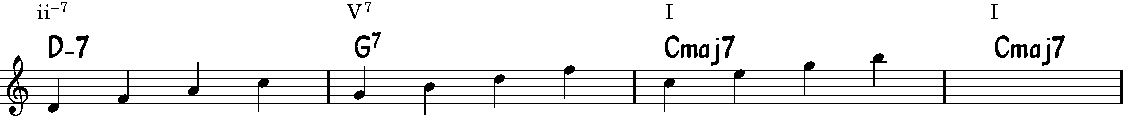
\includegraphics[width=.98\linewidth]{major_ii_v_i.pdf}
\end{center}

\subsection{Minor ii-V-I}
\label{sec:orgae57aa3}

Shortcut, think harmonic minor all the way through. (\flat 3 \& \flat 6)

\begin{center}
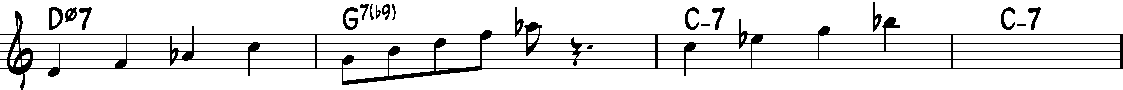
\includegraphics[width=.98\linewidth]{minor_ii_v_i.pdf}
\end{center}

For the half-dim chord, try the Locrian or Locrian nat 2 scales.

\begin{center}
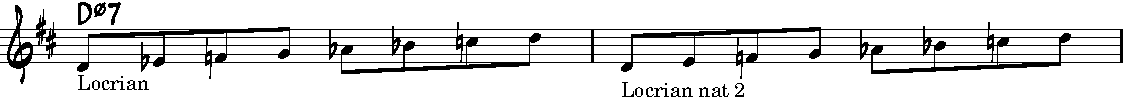
\includegraphics[width=.98\linewidth]{locrian.pdf}
\end{center}

For the G7\flat 9, try the Phrygian Dominant or altered scales.

Usually on a Dom7\flat9 there is a \flat13 (\flat6).

We can think of this as the C harmonic minor (\flat 3 \flat 6) starting on the 5th (G).

The G altered scale starts on G, then every other note is lowered a 1/2 step.

\begin{center}
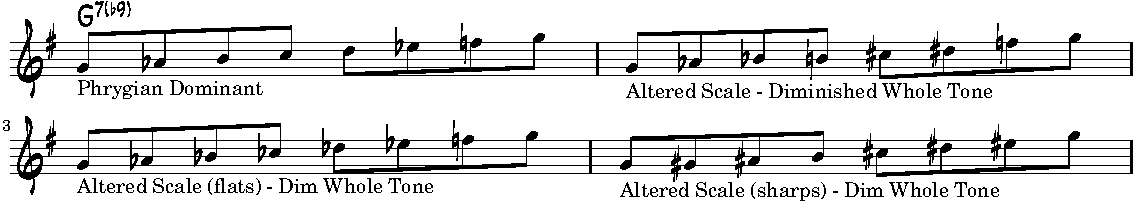
\includegraphics[width=.98\linewidth]{phryg_dom.pdf}
\end{center}

For the Cm7, use the Dorian or melodic minor scales

\begin{center}
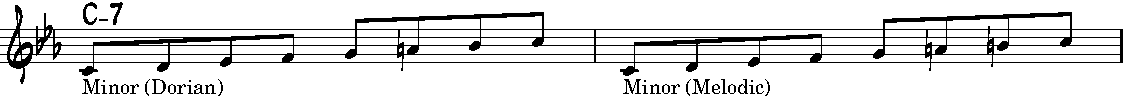
\includegraphics[width=.98\linewidth]{dorian_melodic_minors.pdf}
\end{center}

\subsection{iii-VI-ii-V-I}
\label{sec:orgda6657d}
Can be found in
\begin{itemize}
\item Green Dolphin Street
\item There Will Never Be Another You
\end{itemize}

\begin{center}
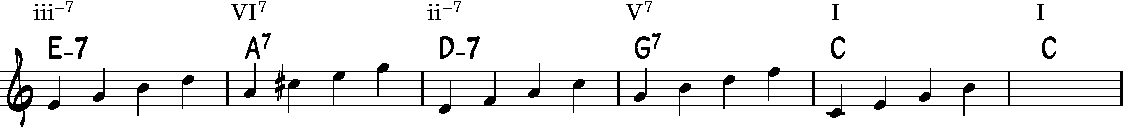
\includegraphics[width=.98\linewidth]{iii-vi-ii-v.pdf}
\end{center}

\subsection{Tritone sub}
\label{sec:org9052300}
Replace the V7 with the V7 a tritone away.

We can also transpose the ii-7 by a tritone.

\begin{itemize}
\item A tritone is a dim 5th (3 whole steps).

\item It is 1/2 way to the octave.
\end{itemize}

\begin{center}
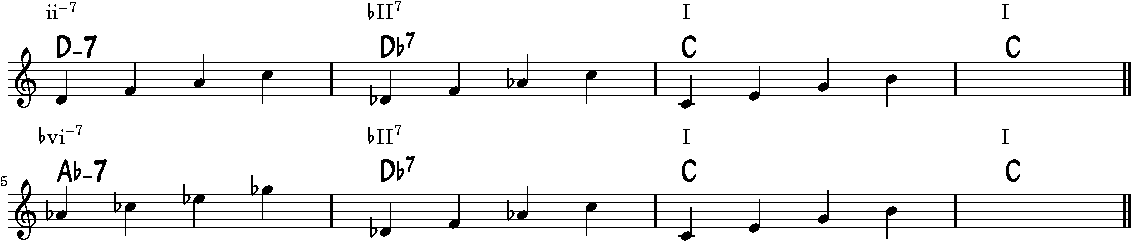
\includegraphics[width=.98\linewidth]{tritone_sub.pdf}
\end{center}

Common notes in substituted chords

\begin{center}
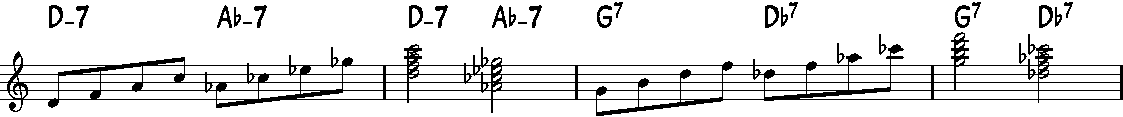
\includegraphics[width=.98\linewidth]{tritone-common-notes.pdf}
\end{center}

\subsection{Backdoor Dominant}
\label{sec:org78d2b9f}

Can also think of this as a minor 3rd sub.

Replace the ii and V chords with chords a m3 higher

\begin{center}
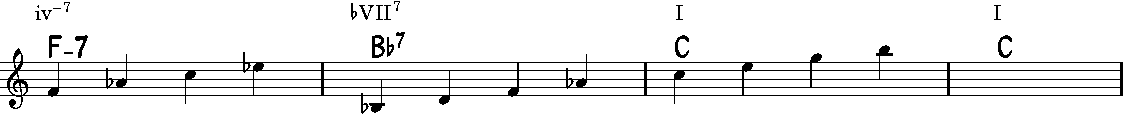
\includegraphics[width=.98\linewidth]{backdoor.pdf}
\end{center}

Notice the common notes in the arpeggios

\begin{center}
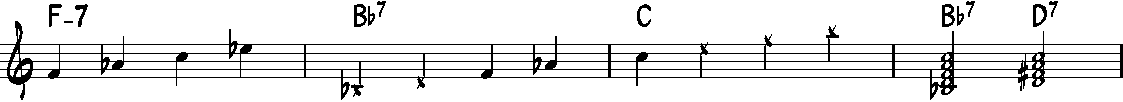
\includegraphics[width=.98\linewidth]{backdoor-common-notes.pdf}
\end{center}

\section{Major ii-V-I phrases}
\label{sec:org5e62f76}
\subsection{In E-flat}
\label{sec:org946466e}

\begin{center}
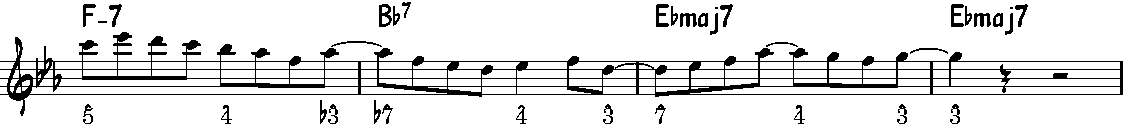
\includegraphics[width=.98\linewidth]{e-flat.pdf}
\end{center}

\subsection{G maj (triplet lead in)}
\label{sec:org81b2040}
\begin{center}
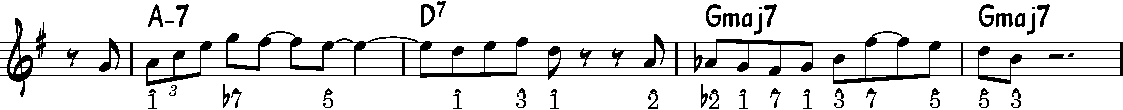
\includegraphics[width=.98\linewidth]{g_maj.pdf}
\end{center}

\subsection{G maj (variation 2)}
\label{sec:orgdc2ce49}
\begin{center}
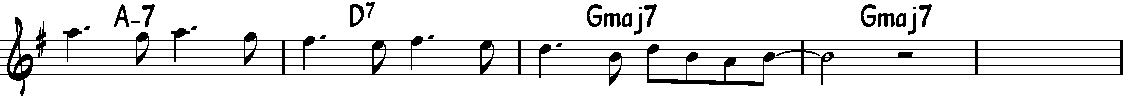
\includegraphics[width=.98\linewidth]{g_maj_v2.pdf}
\end{center}

\subsection{Short ii-V-I in Emaj}
\label{sec:orgdba970a}
\begin{center}
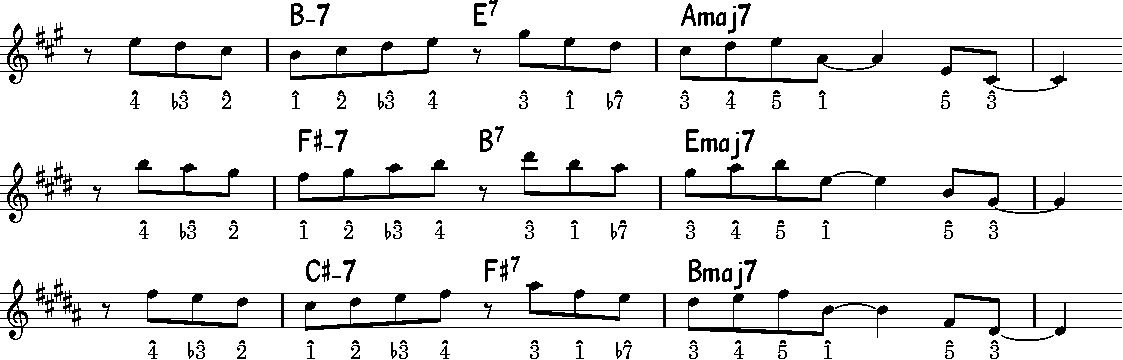
\includegraphics[width=.98\linewidth]{short-ii-v-in-Emaj.pdf}
\end{center}

\subsection{ii-V-I in A maj}
\label{sec:orgb8513ce}
These notes are actually just 1-2-3-5-7 from the major scale.

\begin{center}
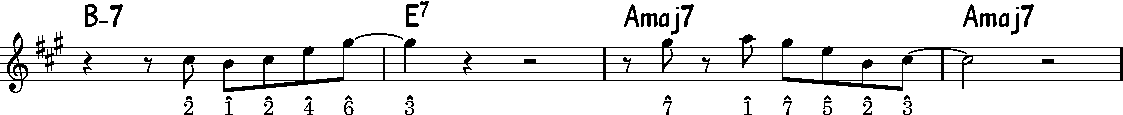
\includegraphics[width=.98\linewidth]{ii-v-in-Amaj.pdf}
\end{center}

\subsection{Dick Oatts - Like someone in Love}
\label{sec:org285f8cf}
This snippet is from m40 (\textasciitilde{}0:51)
Near the beginning of the 2nd chorus

\begin{center}
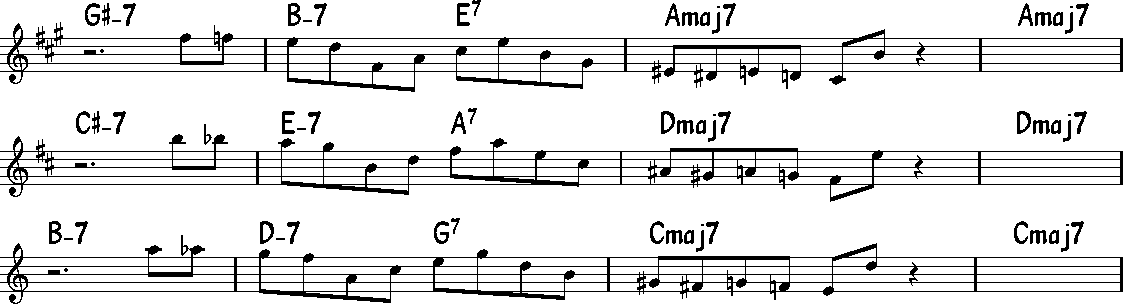
\includegraphics[width=.98\linewidth]{dick_oatts.pdf}
\end{center}

\subsection{In G maj}
\label{sec:orgdaa1ef1}

\begin{center}
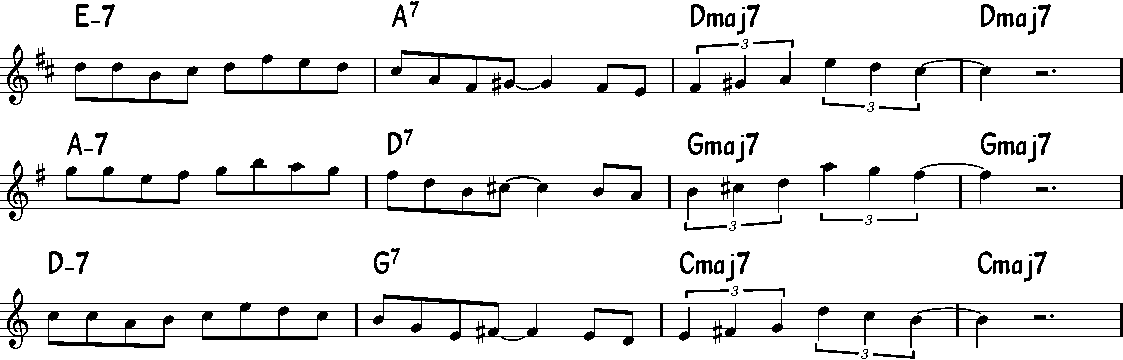
\includegraphics[width=.98\linewidth]{in_g_maj.pdf}
\end{center}

\subsection{In D maj}
\label{sec:orge6532a6}

\begin{center}
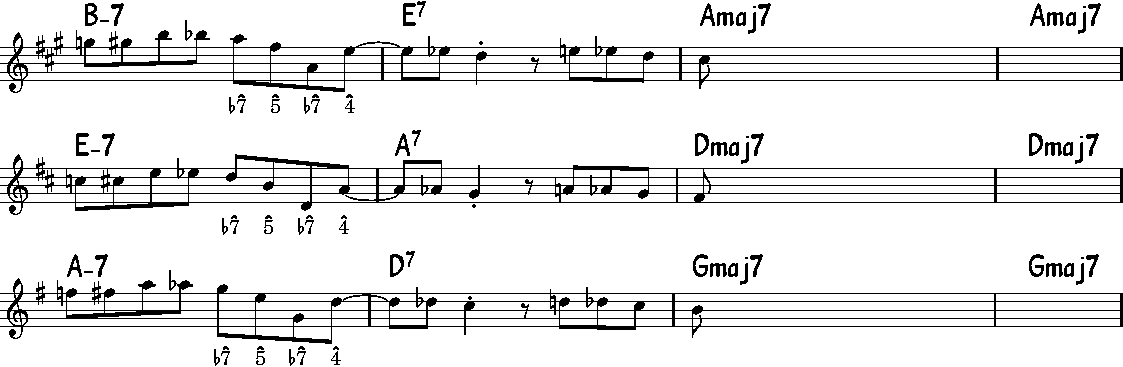
\includegraphics[width=.98\linewidth]{in_d_maj.pdf}
\end{center}

\section{Minor ii-V-i}
\label{sec:org8390d6a}
\subsection{Short minor ii-V in Amin}
\label{sec:orgdaaf764}
\begin{center}
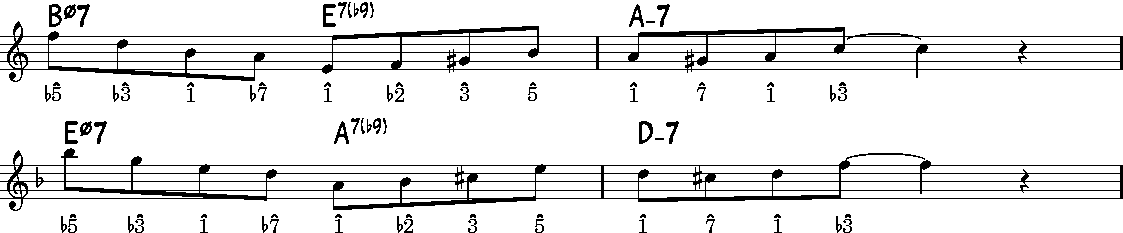
\includegraphics[width=.98\linewidth]{short-ii-v-in-Amin.pdf}
\end{center}

\section{iii-VI-ii-V-I}
\label{sec:org83c45ce}
\section{Tritone sub phrases (Dom chord only)}
\label{sec:org9ce8159}

\subsection{Tritone in Cmaj}
\label{sec:org3f59864}
\begin{center}
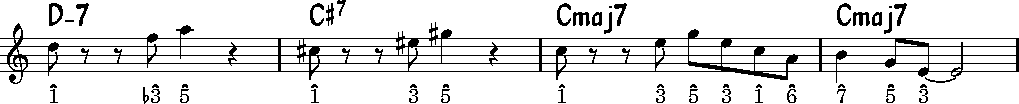
\includegraphics[width=.98\linewidth]{tritone-c-maj.pdf}
\end{center}

\subsection{Tritone Dmaj}
\label{sec:org74ecf25}
\begin{center}
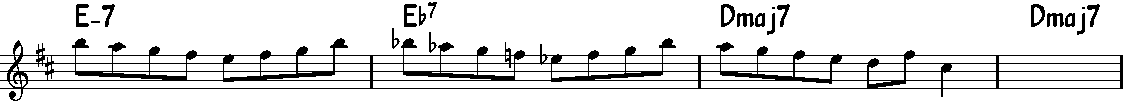
\includegraphics[width=.98\linewidth]{tritone-d-maj.pdf}
\end{center}


\section{Backdoor dominant}
\label{sec:org0febfec}

\subsection{Backdoor 1}
\label{sec:org0014bcf}
\begin{center}
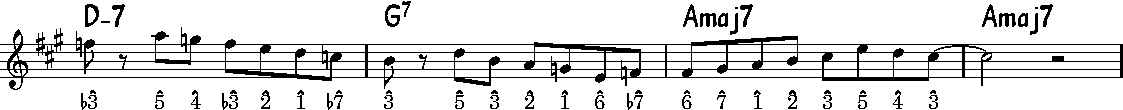
\includegraphics[width=.98\linewidth]{backdoor-1.pdf}
\end{center}
\end{document}
